% Chapter 4 from the standard thesis template
%   that contains an adv. example table and figure.
\chapter{Experimental Setup}

Testing and verification ensures that the new components that we have added to the system are working as intended and has not caused a negative impact on the overall system performance.  To do this, several tests were conducted and verification was obtained by using a well known method of detecting power in a radiometer, a square-law detector.  

Testing began with the square-law detector as this was one of the first components that was obtained.  Next, testing was done with the the software defined radio as a whole.  Finally a cold bath test was done with both the software defined radio and with the square law detector as a system to verify both functionality and to compare the results from both devices.  

In addition to these tests, a few real world tests were also done in the Spring of 2012 and the Spring of 2014.  These tests were conducted by Dr. Brian Hornbuckle's E E 518 class was conducted as part of their lab requirement for the test.  These test results can be found in Appendix 2.

\section{Square-law Detector}
To verify the results that the software defined radio is obtaining, a square-law detector is used to measure the power of the incoming signal.  The incoming signal is split using a power divider so that the signal will be the same to both devices with the exception of the 3 dB plus insertion loss the power divider adds.  This allows us to verify the software defined radio with a proven system.  Square-law detectors have traditionally been used in radiometers and have been proven to work in radiometer applications.  They are also a very simple device which means there is little that can go wrong with using them.


\subsection{Analog Devices ADL5902}

The square-law detector that we obtained is the Analog Devices ADL5902.  The ADL5902 is a true rms responding power detector that has a square law detector, a variable gain amplifier and an output driver. It also has a temperature sensor and will compensate for temperature variations.  The output driver allows for the small signal from the square law detector to be amplified to a level that most analog to digital devices can detect.  This driver however does have low noise and has a noise output of approximately $25nV/ \sqrt{Hz}$ at 100 kHz.  The ADL5902 operates from 50 MHz to 9 GHz and in most cases can detect down to $-60$ dBm.  This works well in our application since the radiometer operates at 1.4 GHz and after the amplification stage we usually see between $-40$ to $-30$ dBm of power.  

The specifications of the ADL5902 can be seen in Table~\ref{data}
shown below.

\begin{table}[h!tb] \centering
\isucaption{ADL5902 Specifications}
\label{ADL5902_data}
% Use: \begin{tabular{|lcc|} to put table in a box
\begin{tabular}{lcc} \hline
\textbf{Parameter @ 900 MHz} & \textbf{Value} & \textbf{Units} \\ \hline
Frequency Range & 50 to 9000 & MHz \\
Dynamic Range & 61 & dB \\
Minimum Input Level, $\pm 1.0$ dB & 60 & dB \\ 
Maximum Input Level, $\pm 1.0$ dB & 1 & db \\
Logarithmic Slope & 53.7 & mV/dB \\ 
Output Voltage Range & 0.03 to 4.8 & V \\ \hline
\end{tabular}
\end{table}

The ADL5902 outputs an analog signal that falls between 0.03 volts and 4.8 volts.  It outputs a change of 53.7 millivolt per dB detected by the ADL5902.  

\subsection{Data acquisition and storage}

In order to analyze the data, a method was developed to acquire the data and store it for later use.  For the N200 software defined radio, this is done automatically by the GNURadio program.  Both the complete signal and the power information is stored to a file for later analysis.  The square-law detector however outputs information as an analog voltage that is linearly proportional to the RF power measured.  This required a system that can capture the analog signal from the ADL5902 and then send the data to be stored.  This was accomplished by using a National Instruments USB-6009 data acquisition unit.  This unit has 8 analog inputs that can sample up to 48 ksps with a resolution of 14-bits.  This was more than adequate for our needs.  To use the USB-6009 a fairly simple Lab View program was created.  This program retrieved the information from the USB-6009 and stored the data in both Lav View's binary format and in a more human friendly ASCII format.  The USB-6009 then connects to a host computer through the USB interface.  This made obtaining the data and using device fairly straightforward to use.

\subsubsection{Lab View Acquisition program}

The Labview program was created to talk to the USB-6009 and then store the data.  In addition, it is able to display in real time the current readings coming from the USB-6009.  This was beneficial during testing of the program but is also good information to have while running an experiment.  

{\begin{figure}[h!tb] \centering
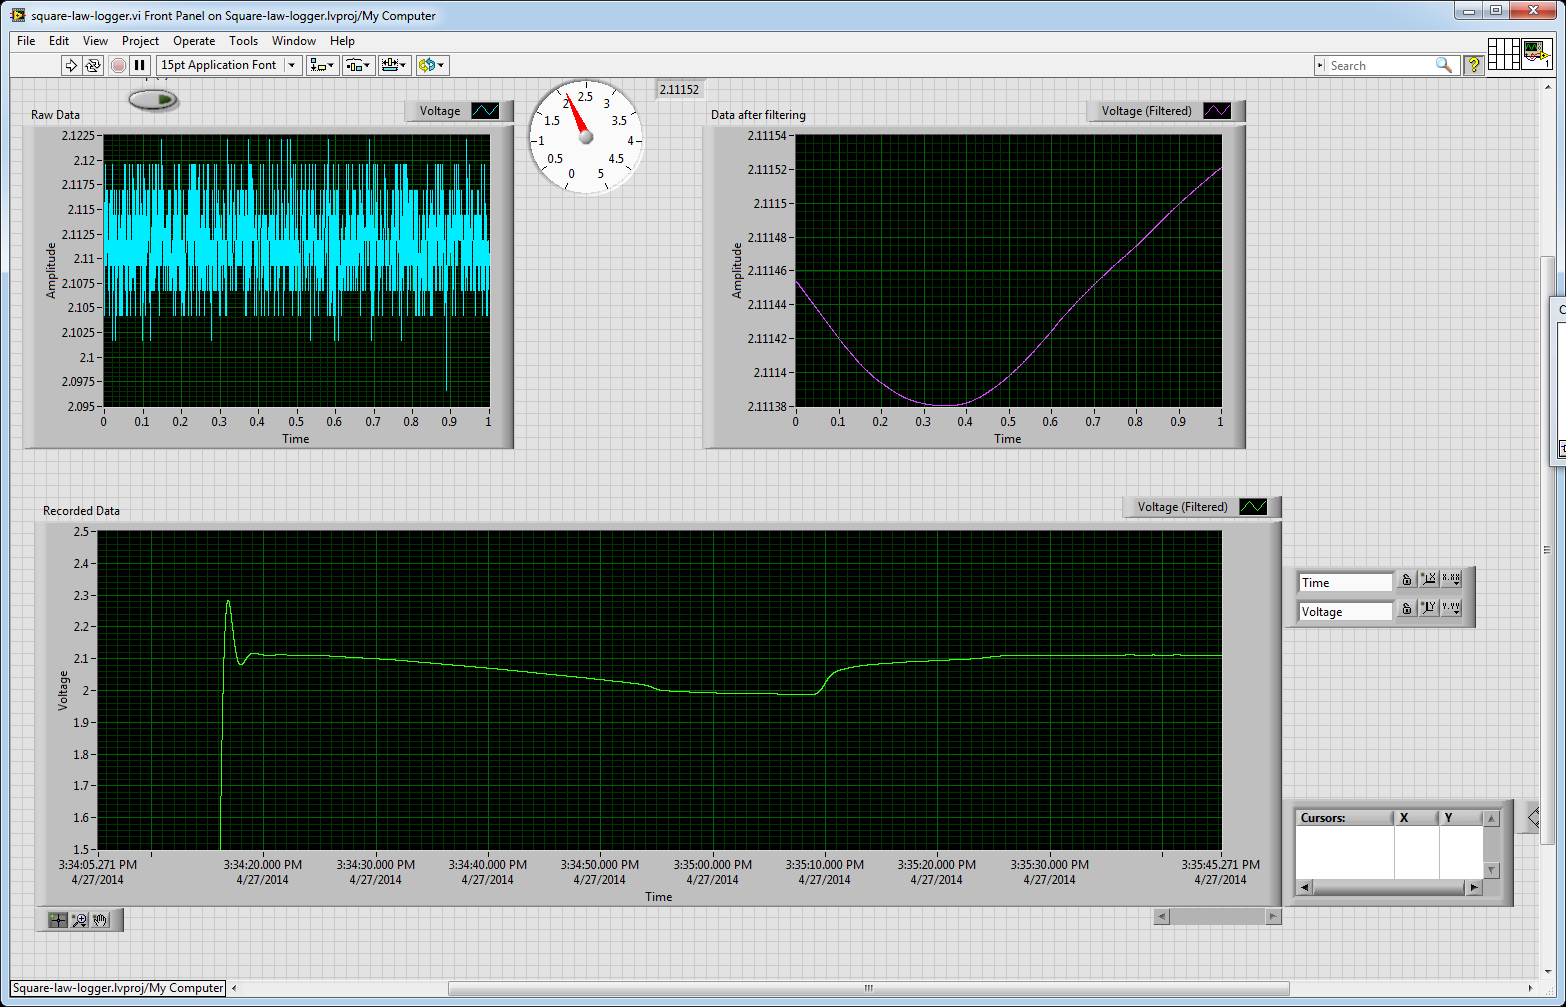
\includegraphics[width=\textwidth]{Images/labviewGUI.png}
\isucaption{A screenshot of the Labview GUI interface}
\label{labviewgui}
\end{figure}
}

The Labview program uses NI's DAQ assitant which allows for quick configuration and setup for the computer to talk to a number of NI devices.  Labview also includes blocks that allows us to easily record the data to a file.  These blocks made up most of the program and resulted in a program that was quickly made.  

While the USB-6009 allows up to 48,000 samples per second, we don't need such a high rate.  A rate of 1,000 samples per second was determined to provide more than enough samples of data.  With such a high rate of samples however, the resulting output will be noisy due to the natural noise found in the RF signal.  Like the software defined radio, we want to filter this noise as well to produce a smoother output.  This was accomplished using a filter block in Labview to help reduce the noise.

{\begin{figure}[h!tb] \centering
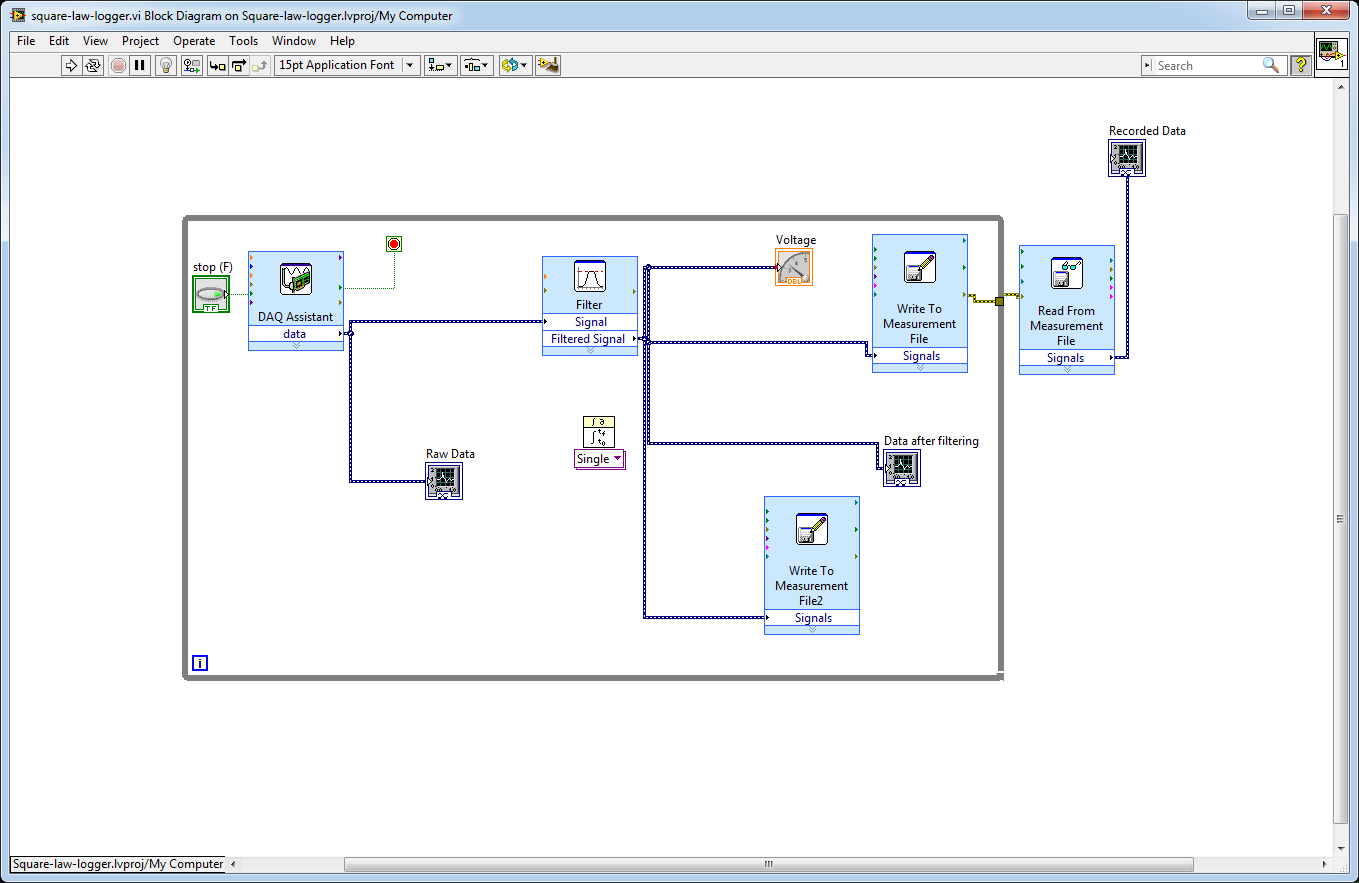
\includegraphics[width=\textwidth]{Images/labview-diagram.png}
\isucaption{A screenshot of the Labview block diagram}
\label{labviewblock}
\end{figure}
}

This program allowed for the data from the square law detector to be easily recorded.  Using Labview also allows us to customize the interface more to our liking and other features such as adding calibration information can also be added as well.  


\subsection{Tests on the ADL5902}
To test the ADL5902 a signal generator was used that had a controlled output.  The specific signal generator that was used was an older model that allowed us to change the output in 10 dBm increments.  The signal generator was also configured for 1.4 GHz as that is the frequency the ISU radiometer is configured to listen at.  Ideally a noise generator would have been desirable, however a noise generator with adjustable power output could not be located on campus.  

The ADL5902 is available from Analog Devices in an evaluation board.  This board pairs the ADL5902 with a AD7466 12-bit analog to digital converter.  This board can then be mated with Analog Devices BlackFin processor which acts as a USB gateway for the AD7466 data.  A test program written in LabView is also provided as well.

The test program provided by Analog Devices allows us to query the ADL5902 and record the raw ADC value.  The test program also allows us to enter in the frequency used during testing and the temperature during the test.  The test program also allows us to calibrate the system as well.  All of the data is then stored into an Excel spreadsheet which can be accessed later.

For this test we used the signal generator set to 1.4 GHz and started at $-60$ dBm for the output signal.  This was selected as this is the lowest the square law detector can detect.  The output power was then incremented on the signal generator in 10 dBm steps.  There was no change to any other parameter.  This was done up to 0 dBm.  Any higher and there was risk of damage to the ADL5902.  This test was then repeated several times and was done with the signal generator stepping up from $-60$ dBm to 0 dBm and from 0 dBm to $-60$ dBm.  

The data collected was then graphed using Excel.  The graph shown in~\ref{adl5902}
Shows that the ADL5902 has a linear output and matches the expected value based on the input.  

\begin{figure}[h!tb] \centering

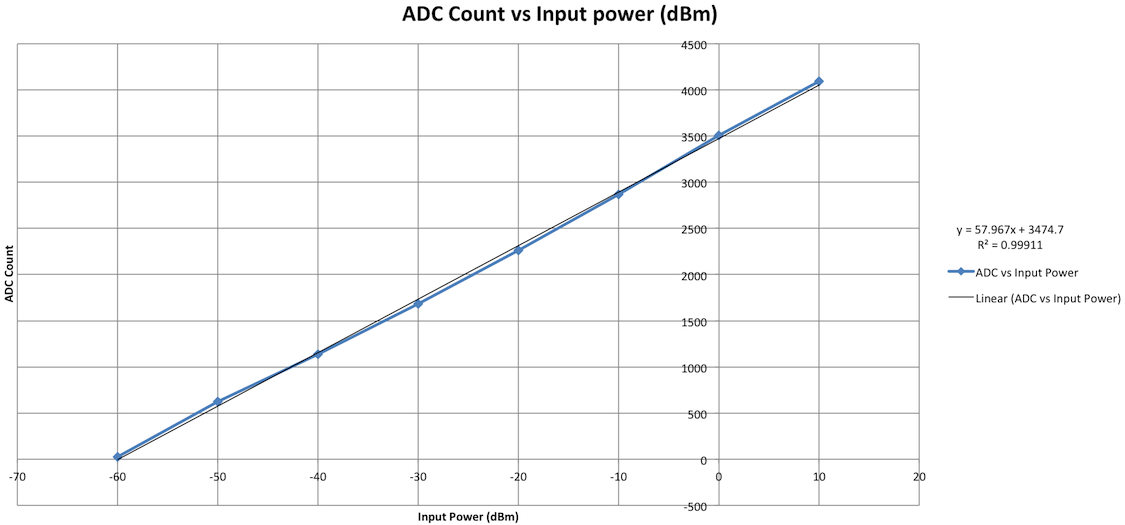
\includegraphics[width=\textwidth]{Images/Linearsquarelaw}

\isucaption{Graph showing the linearity of the ADL5902}
\label{adl5902_linear}
\end{figure}

The ADL5902 test board was considered to be used in the final design for the ISU radiometer and in additional tests.  However, Analog Devices decided to make the information to communicate with the BlackFin processor proprietary and this hampered attempts to integrate that system into our overall system design.  For this reason, it was decided to simply record the analog data that the ADL5902 itself puts out and the PIC32 described above was used to capture and send this information.

\section{Software Defined Radio tests}
Once it was confirmed that the square-law detector was working within the specifications that were given, testing then moved to the software defined radio.  Once the Python program was established for replicating a total power radiometer in software, this was then loaded into GNURadio and used to control the N200 SDR.  GNURadio has a built in noise generator that was then used to test the program and it's ability to measure small changes in noise.  This simulated noise verified that the program written was able to detect changes in noise power using a simulated Gaussian source.  It was desired to also use a hardware based noise generator, however a suitable noise generator could not be located on campus.

\section{Total Power Radiometer Test with Cold Water Bath}
To fully test both the total power radiometer in the software defined radio and the square-law detector, a cold water bath experiment was established to verify that both the square-law detector and SDR was able to measure real world changes in the noise.  In addition, this would also give us a calibration test (confirm this) line to work with.

\subsection{Laboratory Setup}
For this experiment the, ISU radiometer was setup in a laboratory that had access to measurement tools.  To measure the change in noise, a 50 ohm matched load was attached to the radiometer.  The ISU radiometer, with the current filters and LNAs would then amplify and filter the signal.  This signal was then measured by the square-law detector and the N200 SDR.  The 50 ohm load was then submersed into a hot or cold bath.  These water baths were temperature controlled for 100 degrees Centigrade and to 10 degrees Centigrade.  The load was submersed in each bath for 2 minutes to allow for it to reach the same temperature as the bath.  The noise measured was then recorded using GNURadio with the N200 SDR or with the PIC32 setup on the square-law detector.  In addition to the total power measurements, the raw I-Q data was also recorded.  This allowed us to replay the experiment through GNURadio for further study.
\subsection{Test Results}

Several experiments were conducted with this cold-bath configuration to establish that the results were reproducible.  In each case, the experiment showed that both the square-law detector and the SDR were able to measure a change of noise temperature.  Once experiment used a change of only 50 C and the change was easily recorded on the SDR.  Using the experiment described in which the temperatures were held constant, this also gave us a calibration point that we can use to calibrate the radiometer.

\section{Liquid Nitrogen Test}
The Liquid Nitrogen Test was conducted to verify that the radiometer was able to operate within the specifications that were given for the radiometer.  This test is also a fairly common test for testing and calibrating a traditional type of radiometer.  With this test, we can test the radiometer by measuring extreme values for the noise temperature.  To do this, we submerge a matched load attached to the radiometer into a liquid nitrogen bath.  This cools the load, which represents our source, to a physical temperature of approximately 77 Kelvin.  We can then select several "warmer" temperatures such as a ice water bath, room temperature or even boiling water.  Since we expect that the radiometer is linear in how it responds to these noise temperatures, we can then build a calibration line for the radiometer.

\subsection{Testing Apparatus}
To run this test, we need to have some equipment for this.  First and foremost, we need a radiometer.  For this test we used the ISU Radiometer front end, with the LNAs and bandpass filters in place.  The noise diode was turned off for these experiments.  A fifty ohm matched load was then attached to low loss coax and represented our source to the radiometer.  Finally, the output of the radiometer was run to the Ettus N200 software defined radio instead of running the on-board Analog to Digital converter and FPGA.  The data from the N200 was then sent to a MacBook Pro running GNURadio and the custom software that I had written.  This data is sent to the MacBook Pro through a 1 gigabit Ethernet connection due to the large bandwidth coming from the N200.  For these experiments, we only used one "side" of the radiometer.  In theory, both sides of the ISU radiometer should be identical as far as results go.
\subsection{Test Run 1}
The first test run was conducted to help verify that the radiometer was operating correctly and to start to build up data for calibration.  This test was conducted by placing the matched load into the liquid nitrogen bath and then putting it into a ice water bath.  This would give us two points to figure out a calibration point.
\section{Testing with an injected noise source}
This test was designed to test a problem that a software defined radio would be to cope with while a square law detector would not be able to cope with it.  This test injected a known signal at 1.406 GHz to interfere with the normal operation of the radiometer.  In this test, the square law detector, since it is a wide band device, would not be able to accurately measure the change in the total power of the signal.  However, the SDR is able to create a digital filter to filter out the offending signal.  Since this is done in software, the SDR is able to adapt to changes much faster than an analog radiometer.
\subsection{Test setup}
To test this theory, a similar setup was used as with previous tests.  The ISU radiometer's RF front end was once again used to amplify the signal.  One difference however is that a power combiner, which is the same as a power divider, was used to hook up to a signal generator.  The signal generator then provided the offending signal.  By using the signal generator we can control how much power and what frequency the offending signal is at.  In this case we are performing this in a controlled setup and would know ahead of time where the offending signal is.  In the future the SDR defined could identify the offending signal and then filter it out.

Like the other tests, a power divider is used to split the signal after the ISU radiometer RF front end which was then feed to a square-law detector and then the N200 SDR.  The square-law detector was then hooked up to a National Instruments USB-6009 DAQ.  The DAQ was then feed into a labview program to be processed and recorded.  The N200 continued to use the GNURadio program that was created to record the total power coming out.  However, it has been modified with a band reject filter to filter the offending signal.

\subsection{Test results}

insert test results

\section{Further testing}
As discussed earlier, there are some known issues with the RF Front end of the radiometer.  This needs to be explored in more detail or the RF front end may need to be rebuilt.  The issue appears to stem that movement on the RF Front end is causing something to become lose or causes for some local interference to impact the radiometer.  When the radiometer is stationary, it appears to operate normally.  However, as the radiometer is designed to be mounted on a rotational platform and point to the sky for calibration, the movement issue needs to be addressed.  